\chapter[Otimização]{Otimização}

\section{Introdução}
A otimização estrutural se refere a busca de um design estrutural que seja ótimo, ou "o melhor", variando alguns de seus parâmetros estruturais que são pré-estabelecidos. Durante a busca deste design ótimo, o projeto é guiado para satisfazer alguns limites operacionais que são impostos em relação às respostas da estrutura e também por limites nos valores dos parâmentros estruturais que são variados. Segundo \cite{moore1994msc}, a capacidade de otimização de projeto presente no \emph{software} utilizado, \emph{MSC Nastran}, se dá pelo fato de essa otimização ser baseada em uma análise de sensibilidade.

A capacidade de otimização de projeto presente no \emph{software MSC Nastran} é beneficiada, significantemente, devido a análise de sensibilidade. A análise de sensibilidade do projeto computa taxas de variação das respostas da estrutura em relação a variação dos parâmetros de projeto. Esses parâmetros de projeto, ou variáveis de projeto, podem ser espessura de um elemento de placa, comprimento de elemento de barra, raio de perfuração em uma estrutura, propriedades dos materiais, entre outros. No caso a otimização conduzida neste trabalho, os parâmetros de projetos são relacionados à espessura dos elementos de placas e às propriedades dos materias compostos. Essas taxas de variações, ou derivadas parciais na linguagem de cálculo, são chamadas na otimização de coeficientes de sensibilidade de projeto.

Os coeficientes de sensibilidade de projeto são computados explicitamente no \emph{MSC Nastran} e são de extrema importância no processo de otimização, visto que eles podem ser utilizados para prever como uma variação de projeto vai alterar uma resposta da estrutura. Quando estes coeficientes de sensibilidade são aplicados na solução de um otimizador, eles aumentam a eficiência do mesmo, visto que durante a busca para o melhor resultado, o algoritmo sabe não somente o estado atual do projeto, mas também tem uma ideia de qual direção utilizar para buscar o melhor projeto. A capacidade básica de otimização de projeto do \emph{MSC Nastran} depende da existência de informação disponível sobre a sensibilidade do projeto, visto que a otimização não pode ser realizada sem isso.

A utilização de uma otimização se deu com o intuito de encontrar um design ótimo para a estrutura escolhida, além de automatizar o processo utilizando um processo racional e com uma abordagem matemática. A utilização de otimizações se dá em situações como as seguintes:
\begin{enumerate}
  \item Produção de projetos mais eficientes com maiores margens de segurança;
  \item Realização de estudos de variabilidade;
  \item Auxílio em estudos de sensibilidade de projeto;
  \item Validação de dados de testes e resultados de análises (correspondência de modelo).
\end {enumerate}
No caso deste trabalho, o otimizador será primeiramente validado, sendo feita uma otimização de um painel reforçado em material metálico e então uma comparação com a teoria. E em sequeência, após a validação deste otimizador, ele será utiizado para a obtenção de um projeto ótimo para um painel reforçado em material composto.

\section{Análise vs. Otimização de um projeto}
Há algumas diferenças conceituais entre a otmização e a análise de um projeto, ainda que elas possam ser vistas como complementares.

 Durante a realização de uma análise, é criada uma idealização matemática de um sistema físico visando obter respostas de determinadas questões. A clase dessas respostas obtidas depende do tipos de análise que se está buscando, já a precisão dessas respostas, depende da qualidade do modelo e do conhecimento geral do verdadeiro sistema. Portanto, a definição do tipo de elemento finito utilizado, das representações da condições de contorno, dos carregamentos e da malha utilizada, representam um papel extremamente importante em determinar quão bem o modelo está para representar a estrutura física. Logo, o objetivo é obter uma previsão precisa das respostas que são esperadas da estrutura real.

 Em contraste a isso, tem-se o modelo de otimização, no qual idealiza-se mudanças que podem ser feitas na estrutura para melhorar o seu desempenho ou resposta a uma determinada característica. Portanto, para isso, deve-se primeiramente definir o que deseja-se melhorar no projeto, podendo ser como objetivo, por exemplo, uma estrutura com o menor peso possível ou com maior rigidez. Deve-se então estabelecer limites nos quais as variáveis podem flutuar e também expressões de máximos permissíveis, por exemplo.

 A maior diferença portanto entre um modelo de análise e um modelo de otimização é que a análise lida com "a solução", enquanto que a otimização lida com "uma solução". Isto é, durante a performance de uma análise, encontra-se uma única solução, já na perfomance de uma otimização mais de uma solução é possível de ser encontrada. Matematicamente, durante uma otimização o espaço de solução pode conter um mínimo local, mas não necessariamente um mínimo global. Portanto, dependendo das condições iniciais setadas no problema pode-se obter uma solução, já caso essas condições iniciais se alterem, pode-se obter uma solução diferente da obtida anteriormente.

 \section{Princípios básicos de uma Otimização Numérica}
 \subsection{Otimização Numérica - Visão geral}
De acordo com \cite{moore1994msc} a otimização pode ser visto como a seguinte "tarefa de projeto": encontrar um ponto mais baixo em um terreno adjacente. Supõe-se que um indivíduo esteja situado do lado de uma montanha e que deseja encontrar o próximo ponto de menor elevação, este seria o "objetivo". A localização de qualquer ponto será quantificada utilizando as suas coordenadas, logo essas serão as "variáveis de projeto". Supõe-se, também, que existem algumas cercas no terreno, que forçam a restição do espaço de busca ser dentro do território cercado, logo as cercas são as "restrições" que limitam o "espaço de projeto".

Negligenciando a presença de mínimos locais, ou seja, tendo somente um ponto que pode ser considerado como ótimo, achar o ponto de menor elevação dentro deste terreno não é um problema muito grande para um indivíduo comum. Visto que tudo que ele precisará fazer é olhar para a região, e com uma boa perspectiva, apontar qual o ponto mínimo.
No entanto, se pensarmos em um indíviduo que não possui a capacidade de enxergar, o processo de decisão não será tão simples, e isto é basicamente o que ocorre com um otimizador numérico.

Se tratando de um sistema computacional, a determinação do ponto próximo com menor elevação, ou seja, o valor da função objetivo, deverá ser feita utilizando análises numéricas. Portanto, necessita-se de um método sistemático para solucionar tais problemas e para isso tem-se diversas técnicas, chamadas de algoritmos de otimização numérica. Genericamente, os métodos de otimização numérica visam determinar a "direção da busca", o que permite encontrar um ótimo que obedeça as restrições estabelecidas.

Visando encontrar a "direção de busca", deve-se determinar o valor do gradiente da função objetivo e então, utilizar essa informação para estabelecer uma provável direção. No exemplo citado, de encontrar um ponto próximo com menor elevação, mesmo para um indivíduo privado de vista, é possível encontrar a direção dando passos pequenos, por exemplo, até encontrar as cercas como restrições e ir estabelecendo as diferenças nas elevações de cada passada. Este tipo de otimização que utiliza a ideia do gradiente é chamada, portanto, de método baseado no gradiente. E dentro deste método a ideia é repetir o processo de busca até que não seja mais possível reduzir a função objetivo.

\subsection{Otimização Numérica - Visão quantitativa}
Em uma visão quantitativa de uma otimização numérica, tem-se portanto, que deve-se encontrar o valor de \emph{\textbf{X}} que minimize ou maximize, dependendo do problema, a função objetivo \emph{F(\textbf{X})} submetida à:

\begin{enumerate}
\item Restrições de desigualdade
\begin{equation} \label{otimization_1}
\begin{split}
g_{j}(\textbf{X})\leq0 \\
j = 1, ..., n_{g}\\
\end{split}
\end{equation}
\item Restrições de igualdade
\begin{equation} \label{otimization_2}
\begin{split}
h_{k}(\textbf{X})=0 \\
k = 1, ..., n_{h}\\
\end{split}
\end{equation}
\item Restrições laterais
\begin{equation} \label{otimization_3}
\begin{split}
x_{i}^L \leq x_{i}\leq x_{i}^U  \\
i = 1, ..., n\\
\end{split}
\end{equation}
\item Variáveis de projeto
\begin{equation} \label{otimization_4}
\textbf{X} = {x_{1}, x_{2}, ..., x_{n}}
\end{equation}

\end {enumerate}

Nesta notação abordada, tem-se que \textbf{X}, em maiuscúlo e negrito, é um vetor, enquanto as outras variáveis, em minúsculo, são membros deste vetor. E tem-se como função objetivo a quantidade escalar a ser minimizada. As restrições laterais são utilizadas como as variáveis de projeto para limitar a região de busca, e as restrições de desigualdade, convencionamente, são expressas na forma de menor ou igual a zero. E as restrições de igualdade, caso existam, devem satisfazer o \emph{design} "ótimo".

\subsection{Busca numérica por um ótimo}
A solução de otimização utilizada pelo \emph{software MSC Nastran} durante o desenvolvimento deste estudo é referenciada como: Método baseado no gradiente.

O primeiro passo, em um procedimento numérico, é determinar a direção de busca. Este procedimento de busca é repetido até o ponto no qual não consegue obter melhorias na função objetivo sem violar as restrições. Em um contexto de otimização estrutural, a situação pode-se complicar sendo considerada com inviável (uma ou mais restrições são violadas), ou crítica (ponto situado exatamente nas restrições).

A ideia de utilizar o gradiente como base para a otimização, ou seja, dar pequenos passos nas diversas direções das variáveis de projeto, corresponde exatamente ao conceito matemático de diferenças finitas, que é dado por:

\begin{equation} \label{otimization_5}
\frac{d\emph{f}(x)}{dx} = \dfrac{\emph{f}(x + \Delta x)-f(x)}{\Delta x}
\end{equation}
Onde ${\Delta x}$ representa as pequenas variações, pequenos passos, dados na direção \emph{x}. E na maioria dos casos, é considerado um vetor de variáveis de projeto, logo, o vetor gradiente resultante pode ser escrito em função das derivadas parciais conforme:
\begin{equation} \label{otimization_6}
\nabla F(X) =
\begin{bmatrix}
    \frac{d\emph{f}(x)}{dx_1} \\
    \vdots\\
    \frac{d\emph{f}(x)}{dx_n}
\end{bmatrix}
=
\begin{bmatrix}
    \dfrac{\emph{f}(X + \Delta x_1)-F(X)}{\Delta x_1}\\
    \vdots\\
    \dfrac{\emph{f}(X + \Delta x_n)-F(X)}{\Delta x_n}
\end{bmatrix}
\end{equation}

Fisicamente, o vetor gradiente aponta na direção de aumento da função objetivo. Portanto, se quiser minimizar a função objetivo, deve-se mover na direção oposta daquele gradiente e o vetor de busca \textbf{S} é dado por:

\begin{equation} \label{otimization_7}
S = \nabla F
\end{equation}

O \emph{software MSC Nastran} utiliza este método quando nenhuma das restrições são críticas ou violadas e somente do ponto inicial para outros. Embora esta direção de busca seja uma boa direção inicial, subsequente direções de busca, utilizando este método, não funcionam propriamente para melhorar a função objetivo. Portanto, o \emph{software MSC Nastran} utiliza métodos mais eficientes que podem ser generalizados para casos de restrições ativas e/ou violadas, que são as condições de Kuhn-Tucker em conjunto com o algoritmo de determinação da direção de busca.

\subsubsection{Condições de Kuhn-Tucker}
Considerando um espaço para as variáveis de projeto, com as restrições $g_1(X)$ e $g_2(X)$ e uma função objetivo F(X), conforme mostrado na  \autoref{fig_KuhnTucker1}.

\begin{figure}[h]
	\caption{\label{fig_KuhnTucker1}Condições de Kuhn-Tucker em um ótimo restrito.}
  \centering
  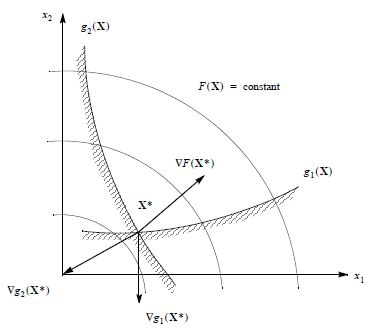
\includegraphics[scale=0.71]{figura/KuhnTucker1}
	\legend{Fonte: \cite{moore1994msc}}
\end{figure}
\

Os limites das restrições são as curvas nas quais os valores das restrições são identicamente iguais a zero. O ponto ótimo, nesta na \autoref{fig_KuhnTucker1}, é o ponto na interseção das duas curvas de restrições (ponto X*). Caso os gradientes das duas curvas de restrições sejam computados, observa-se que eles apontam em diferentes direções, visto que os gradientes apontam na direção de crescimento do valor da função. Portanto, para essa situação de um ótimo restrito, as condições de Kuhn-Tucker estabelecem que o vetor soma da função objetivo e das restrições devem ser iguais a zero, dados apropriados fatores multiplicativos (multiplicadores de Lagrange). A \autoref{fig_KuhnTucker2} mostra a situação em que os multiplicadores de Lagrange $\lambda_1$ e $\lambda_2$ fazem com que o vetor soma seja zero.

\begin{figure}[h]
	\caption{\label{fig_KuhnTucker2}Interpretação gráfica das condições de Kuhn-Tucker.}
  \centering
  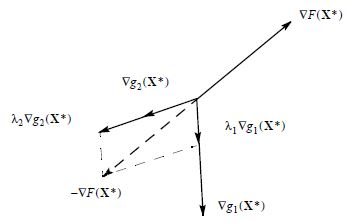
\includegraphics[scale=1.0]{figura/KuhnTucker2}
	\legend{Fonte: \cite{moore1994msc}}
\end{figure}

\section{Otimização Estrutural}
Durante a realização de uma análise estrutural, o objetivo é construir uma idealização matemática de um determinado sistema físico. Para isso, deve-se portanto, determinar as propriedades da análise, o tipo de resposta que será obtida e também uma malha em elementos finitos que será capaz de computar as respostas de maneira acurada. As propriedades da análise consistem em definir os materiais, as espessuras dos elementos, as malhas dos elementos, entre outras variáveis, e os tipos de respostas podem ser, por exemplo, tensões ou deformações nos elementos, frequências modais e outros. Já durante a realização de uma otimização, deseja-se definir como o modelo varia, em busca de um design melhor, com a alteração das variáveis de otimização.

A otimização utilizada pelo \emph{software MSC Nastran} conecta portanto as duas propostas acima utilizando conceitos intermediários:
\begin{enumerate}
\item Propriedades de projeto: proporcionam uma conexão entre as variáveis de projeto utilizadas pelo otimizador e as propriedades dos elementos utilizadas pela análise em elementos finitos;
\item Respostas de projeto: é um resultado físico que pode ser utilizado como um objetivo de projeto ou, seguindo imposições do usuário, como uma restrição de projeto.
\end{enumerate}

\subsection{Conexão entre análise estrutural e otimização numérica}
As primeiras tentativas utilizadas para conectarem a análise estrutural com a otimização numérica se baseavam na ideia de um acoplamento direto, chamado também de \emph{"black box"}, conforme mostrado na \autoref{fig_blackbox}.

\begin{figure}[h]
	\caption{\label{fig_blackbox}Acoplamento direto ou \emph{"black box"}.}
  \centering
  \includegraphics[scale=0.7]{figura/blackbox}
	\legend{Fonte: \cite{moore1994msc}}
\end{figure}

\
Neste método, todas as vezes que o otimizador necessitase de uma avaliação da função objetivo seria realizada uma análise em elementos finitos. Este método, portanto, se mostrou inviável mesmo para problemas pequenos, visto que necessitaria de muitos recursos computacionais. O principal fator relacionado à otimização estrutural que torna a ideia do \emph{"black box"} inviável, é que as respostas quantitativas de interesse são normalmente funções implícitas das variáveis de projeto. Isto é, por exemplo, a variação de tensão em um elemento de placa em função da variação da espessura da mesma, só pode ser obtido realizando uma análise em elementos finitos da estrutura.

Portanto, para evitar que seja feita uma análise em elementos finitos para cada variação durante a otimização numérica, o \emph{MSC Nastran} utiliza o conceito de realizar aproximações, conforme \autoref{fig_blackbox2}.

O conceito das aproximações baseia-se principalmente na ideia de reduzir or problema suficientemente, de maneira que, somente as informações mais pertinentes sejam consideradas no processo de geração do melhor projeto. Uma vez que um novo design é proposto pelo otimizador, baseado na informação fornecida pelo modelo aproximado, o próximo passo é realizar uma análise mais detalhada em elementos finitos da nova configuração. E com isso, é possível checar se o novo design realmente satisfaz as restrições de projeto e reduz a função objetivo. Se uma subsequente otimização ainda for necessária, a análise em elementos finitos serve como base para construir um submodelo com aproximações. E portanto, estes ciclos de projetos são repetidos até que a convergência seja atingida.

\begin{figure}[h]
	\caption{\label{fig_blackbox2}Acoplamento entre análise em elementos finitos e otimização numérica utilizando aproximações.}
  \centering
  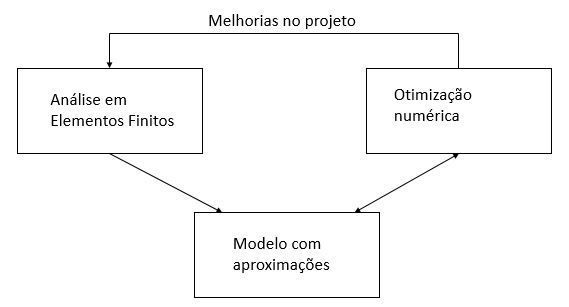
\includegraphics[scale=0.7]{figura/Blackbox2}
	\legend{Fonte: \cite{moore1994msc}}
\end{figure}

\subsection{Conceitos fundamentais}
Dentro da otimização estrutural do \emph{MSC Nastran} há alguns conceitos fundamentais que devem ser destacados, conforme segue.

\subsubsection{Variáveis de projeto}
As variáveis de projeto são quantidades que são conhecidas pelo otimizador e que podem ser diretamente alteradas para satisfazerem a proposta da otimização. No \emph{MSC Nastran}, as variáveis de projeto são definidas pela entrada do tipo DESVAR e elas só afetam a análise em elementos finitos caso sejam conectadas com as propriedades de projeto e/ou respostas de projeto.

É função do usuário definir os limites de variação das variáveis de projeto, ou seja, impor as restrições. O \emph{MSC Nastran} é capaz de distinguir entre variáveis de projeto dependentes e independentes, e também é capaz de utilizar o conceito de variáveis discretas, onde o valor das variáveis é restrito a um específico \emph{set} de números reais.

No caso deste estudo, as variáveis de projeto, detalhadas na seção do Desenvolvimento, são as espessuras do revestimento e do reforçador, e também os parâmetros de laminação ($\xi$).

\subsubsection{Propriedades de projeto}
As propriedades de projeto são quantidades que influenciam diretamente na análise de elementos finitos e que incluem propriedades como espessuras, materiais, densidades e posicionamento dos nós.

As propriedades dos elementos variam de acordo com o tipo de elemento utilizado no modelo, conforme mostrado na \autoref{fig_designprop}. Bem como as propriedades dos materiais, dependem do tipo de entrada de material que será fornecida.

\begin{figure}[h]
	\caption{\label{fig_designprop}Exemplos de propriedades dos elementos e propriedades do materiais.}
  \centering
  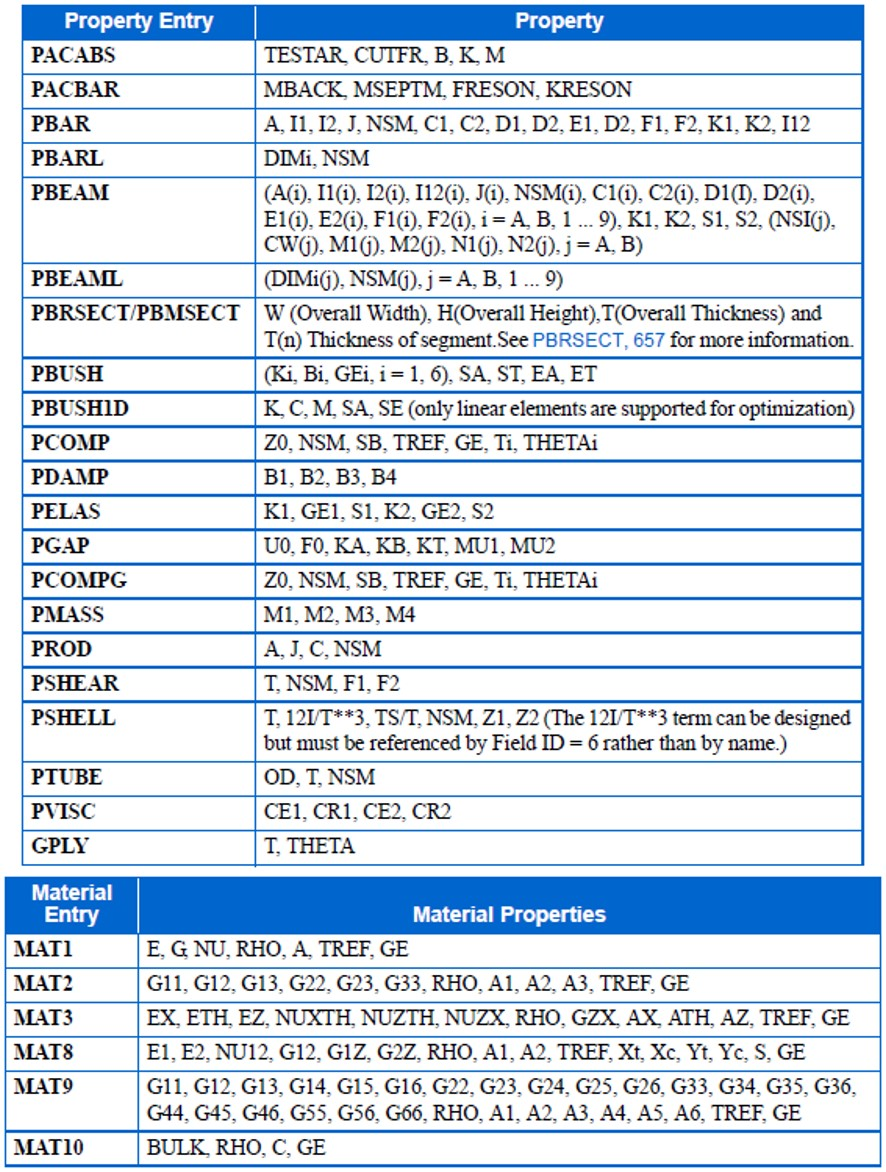
\includegraphics[scale=0.5]{figura/DesignProp}
	\legend{Fonte: \cite{moore1994msc}}
\end{figure}

No caso deste estudo, detalhado na seção do Desenvolvimento, propriedades de elementos do tipo PSHELL e propriedades dos materiais do tipo MAT2 foram utilizadas para gerar o modelo.

\subsubsection{Respostas de projeto}
As respostas de projeto são utilizadas no \emph{MSC Nastran} como bases para definirem o objetivo e as restrições de projeto. Assim como as propriedades de projeto, as respostas de projeto funcionam como uma conexão entre a análise em elementos finitos e a otimização numérica, e podem ser divididas em três tipos.

\begin{enumerate}
\item Resposta tipo 1: essas respostas são obtidas diretamente de uma análise do \emph{MSC Nastran} e utiliza-se DRESP1 para acessá-las. Exemplos: peso estrutural, deslocamentos de nós e tensões nos elementos.
\item Resposta tipo 2: esse tipo de resposta permite que o usuário utilize uma equação para manipular as respostas do tipo 1 e utiliza-se DRESP2 para acessá-las. Permite, por exemplo, que o usuário formule critérios de falha, avalia o comportamento referente a flambagem, imponha limitações para as respostas, entre outros.
\item Resposta tipo 3: este tipo de resposta é semelhante ao tipo 2, mas permite que o usuário utilize o API (\emph{Application Programming Interface}) para buscas processos externos ao \emph{MSC Nastran}. Utiliza-se DRESP3 para acessá-las.
\end{enumerate}

No caso deste estudo, detalhado na seção do Desenvolvimento, as respostas de projeto do tipo 1 e 2 (DRESP1 e DRESP2) foram utilizadas no modelo.

\subsubsection{Restrições de projeto}
As restrições de projeto são acessadas utilizando o DCONSTR para identificarem um resposta (DRESP1, DRESP2 ou DRESP3) e assim, impor um limite a essa resposta.
\begin{equation} \label{otimization_constraints}
r_{j}^L \leq r_{j}(X)\leq r_{j}^U
\end{equation}

onde $r_{j}^L$ é o limite inferior da j-ésima resposta e $r_{j}^U$ é o limite superior.

\subsubsection{Função objetivo do projeto}
A função objetivo do projeto é uma quantidade escalar que deve ser minimizada ou maximizada pelo otimizador, dependendo do problema proposto. Esta função objetivo é selecionada utilizando o comando DESOBJ e este comando referencia a alguma resposta do tipo DRESP1, DRESP2 ou DRESP3 que deve ser uma resposta escalar simples.

No caso deste estudo, detalhado na seção do Desenvolvimento, a função objetivo é minimizar o peso da estrutura. Para isso, utiliza-se de três soluções do \emph{MSC Nastran}, a solução de otimização (SOL 200), a solução estática (SOL 101) a solução de flambagem (SOL 105). 
